%\documentclass[11pt]{jarticle}
\documentclass[11pt]{ujarticle} %%uplatexを用いる際はこちらを使用
\usepackage{fundsx}
\usepackage{url}
\usepackage[dvipdfmx]{graphicx}

\title{データサイエンス演習 最終レポート\\＜レポートのタイトル＞}

\author{% 
＜グループ番号・グループ名＞\\
＜学籍番号・名前（姓 名）＞\\
＜学籍番号・名前（姓 名）＞\\
＜学籍番号・名前（姓 名）＞\\
＜学籍番号・名前（姓 名）＞
}
\date{提出日 ＜提出日＞}

\begin{document}

\maketitle
\clearpage

\section{概要}
＜本レポートの概要を記述する．記述例：本グループではxxxを目的として，（xxxに着目し）xxxという仮説を立て検証した．検証にはxxx手法を用い，xxxデータセットによりモデルの訓練を行い，テストデータにて検証した結果，xxxであった．＞

\section{背景・⽬的}
＜ここに社会問題や社会背景，それによって導かれた目的や着目した要因，他の関連研究や他に検討した内容等を記述する．＞

\section{対象としたデータセット}
＜ここに，対象としたデータセットについての説明を書く．データセットの内容，特徴，出自（どこからもってきたのか），データを構成する属性，データの量を記述する．データの一部を，図として掲示することが望ましい．＞

% URLを記述する際は，\url{https://..../}のようにするとよい

\section{⼿法}
＜ここに機械学習の具体的な手法名やその簡単な説明，また前処理後処理の内容等を記述する．全体の流れを説明するような図があると理解しやすい．可視化等で工夫した点はこちらにまとめても良い．

% 図番号は図\ref{fig:1}のように記載する

\begin{figure}[htbp]
    \centering
    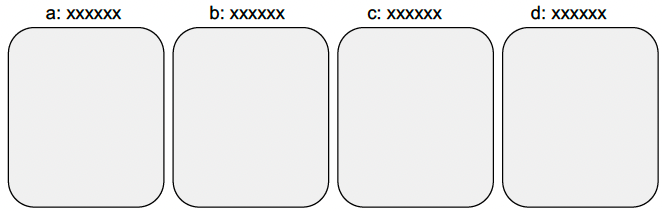
\includegraphics[width=1.0\linewidth]{sample.png}
    \caption{全体の流れ．a: データセットの取得および前処理．b: モデルの訓練．c: 訓練したモデルによる推論．d: 推論結果のxxxへの応⽤＞}
    \label{fig:1}
\end{figure}


\section{実装（実験）}
＜実験環境や条件を記述する．内容はローカルで行った場合はコンピュータのモデル名やCPU等の諸元，クラウドの場合は出典の記載も忘れずに．データ取得前と前処理後の状態，訓練・テストデータセットの具体的な数，訓練時間，モデルの評価方法，代表的なパラメータの値など．必要であれば図も忘れずに．
記述例：Google Colaboratory\cite{ref:1}のPython3.xカーネルを用い，モデルはライブラリscikit-learnのxxxを用いた．可視化やユーザインタフェースにはProcessing\cite{ref:2}を用いた．

グループにおける作業の分担は，AさんがGoogle Colaboratory でのコーディングを主に担当し，Bさんはscikit-learnの使い方を中心にAさんのコーディングをサポートした．CさんはProcessingによる可視化とユーザインタフェースの部分を担当し，DさんとEさんは実験に用いるデータ収集を担当した．（※この段落はグループ内で記述を共有した）＞

\section{結果}
＜上の実装から得られた結果（訓練経過のプロットや，テストデータを用いた評価，推論結果等）をここに記述する．プロットはタイトル，縦軸，横軸，複数条件であればレジェンド（凡例）を忘れずに．＞

\section{結論･考察}
＜この章については，400字以上，個々人で記述する場合は氏名を明記の上、ひとり150文字以上．

やったことのまとめ，実験結果から得られた結論等を記述する．苦労した点や今後の展望等あれば見出し付きで記述すると読みやすい．＞



% 参考⽂献
\begin{thebibliography}{99}
% ＜
 \bibitem{ref:1} 著者名，文献のタイトル，文献の出典名（論文誌，国際会議，学会名），（必要に応じ）Vol.をつけて巻，No.をつけて号，pp.をつけて始めのページ-終わりのページ，西暦年．
 \bibitem{ref:2} 著者名，文献のタイトル，文献の出典名（論文誌，国際会議，学会名），（必要に応じ）Vol.をつけて巻，No.をつけて号，pp.をつけて始めのページ-終わりのページ，西暦年．
% ＞
\end{thebibliography}

\clearpage
\section*{実験に⽤いたソースコード}

解析に用いたスクリプトのうち，本研究の手法を特徴づける部分を抜粋する．
全体は \url{https://github.com/KurenNagata/bravo} に置いてある．

\subsection*{A. 実プレー時間の復元（\texttt{extract\_dataset.py}）}

イベントに記録された継続時間をつなぎ，10秒を超える空白を停止とみなして時計から除く．
これにより，前後の「3分」を停止時間の混入なくそろえられる．

\begin{verbatim}
MAX_LIVE_GAP_SEC = 10.0

def live_segments(events, period):
    """possession 内のイベント列から実プレー区間を復元する。"""
    by_possession = defaultdict(list)
    for e in events:
        if e["period"] != period or "possession" not in e:
            continue
        if e["type"]["name"] in NON_PLAY_TYPES:
            continue
        s = float(tsec(e))
        duration = max(0.0, float(e.get("duration", 0.0) or 0.0))
        by_possession[e["possession"]].append((s, s + duration))

    pieces = []
    for intervals in by_possession.values():
        intervals.sort()
        cur_s, cur_t = intervals[0]
        for s, t in intervals[1:]:
            if s - cur_t > MAX_LIVE_GAP_SEC:   # 10秒超の空白は停止
                if cur_t > cur_s:
                    pieces.append((cur_s, cur_t))
                cur_s, cur_t = s, t
            else:
                cur_t = max(cur_t, t)
        if cur_t > cur_s:
            pieces.append((cur_s, cur_t))

    pieces.sort()
    merged = []
    for s, t in pieces:
        if not merged or s > merged[-1][1]:
            merged.append((s, t))
        else:
            merged[-1] = (merged[-1][0], max(merged[-1][1], t))
    return merged
\end{verbatim}

\subsection*{B. 32項目の組み立て（\texttt{train\_models.py}）}

イベントの記録から機械的に列挙した項目を，内容・位置，実プレー1分あたりの回数，
テンポの3種類に分けてまとめる．指標を人が選び直さないための処理である．

\begin{verbatim}
def feature_sets(all_cols):
    per_active_min = [c for c in all_cols
                      if c.endswith("_per_active_min")]
    raw_counts = [c for c in all_cols
                  if (c.startswith("n_") or c == "xg_sum")
                  and not c.endswith("_per_active_min")]
    tempo = [
        "events_per_possession",
        "passes_per_possession",
        "within_possession_gap_mean",
    ]
    content = [c for c in all_cols
               if c not in per_active_min
               and c not in raw_counts
               and c not in tempo]
    return {
        "flow_full": content + per_active_min + tempo,  # 32項目
        "content_only": content,
    }
\end{verbatim}

\subsection*{C. fold先行の対応づけ（\texttt{did\_foldfirst.py}）}

試合を先に5つの組へ分け，対応づけを同じ組の中だけで行う．
これにより，同じ試合・同じ対が学習と評価にまたがらないことを設計だけで保証する．

\begin{verbatim}
def match_within_blocks(treated, controls, block_of, use_xg):
    used, pairs = set(), []
    order = sorted(range(len(treated)),
                   key=lambda i: treated[i]["clock"])
    for i in order:
        t = treated[i]
        if use_xg and t.get("xg") is None:
            continue
        tb = block_of[str(t["match_id"])]
        best_j, best_cost = None, None
        for j, c in enumerate(controls):
            if j in used or block_of[str(c["match_id"])] != tb:
                continue                    # 同じ組の中だけで探す
            if c["period"] != t["period"]:
                continue                    # 前後半を一致
            if c["state"] != t["state"]:
                continue                    # 点差状態を一致
            if c["is_home"] != t["is_home"]:
                continue                    # ホーム／アウェーを一致
            if c["match_id"] == t["match_id"]:
                continue
            gap = abs(c["clock"] - t["clock"])
            if gap > MATCH_MINUTE_TOL:       # 時刻差 8 分以内
                continue
            cost = gap / MATCH_MINUTE_TOL
            if use_xg:
                if c.get("xg") is None:
                    continue
                dxg = abs(c["xg"] - t["xg"])
                if dxg > XG_TOL:             # xG 差 0.10 以内
                    continue
                cost += dxg / XG_TOL
            if best_cost is None or cost < best_cost:
                best_j, best_cost = j, cost
        if best_j is not None:
            used.add(best_j)
            pairs.append((t, controls[best_j]))
    return pairs
\end{verbatim}

\subsection*{D. 差の差の学習・評価（\texttt{did\_foldfirst.py}，\texttt{train\_models.py}）}

後区間と前区間の差を入力とし，組をそのままfoldとして交差検証する．
AUCは対になった処置側・対照側の判定値の大小から求め，
95\%信頼区間は連結成分を単位とするブートストラップで与える．

\begin{verbatim}
# 判別器（train_models.py）
Pipeline([
    ("impute", SimpleImputer(strategy="median")),
    ("scale", StandardScaler()),
    ("clf", LogisticRegression(max_iter=2000, C=1.0,
                               random_state=SEED)),
])

# 学習・評価（did_foldfirst.py の evaluate_blocks より抜粋）
rows = []
for t, c in pairs:
    block = block_of[str(t["match_id"])]
    for label, u in ((1, t), (0, c)):
        delta = {f: (u["after"][f] - u["before"][f])   # 後 - 前
                 for f in cols}
        rows.append({"block": block, "pair": t["key"],
                     "label": label, **delta})
df = pd.DataFrame(rows)

probs = np.empty(len(df))
for b in range(N_BLOCKS):              # 組をそのまま fold にする
    te = df["block"] == b
    model = build_models()[PRIMARY_MODEL].fit(
        df.loc[~te, cols].to_numpy(dtype=float),
        df.loc[~te, "label"].to_numpy())
    probs[te.to_numpy()] = model.predict_proba(
        df.loc[te, cols].to_numpy(dtype=float))[:, 1]

piv = df.assign(prob=probs).pivot_table(
    index="pair", columns="label", values="prob").dropna()
values = piv[[0, 1]].to_numpy()
observed = roc_auc_score(np.tile([0, 1], len(values)),
                         values.reshape(-1))

# 連結成分を単位としたブートストラップ 5,000 回
rng = np.random.default_rng(SEED)
boots = np.empty(N_BOOT)
for b in range(N_BOOT):
    pick = rng.choice(keys, size=len(keys), replace=True)
    idx = [i for cmp_ in pick for i in by_comp[cmp_]]
    boots[b] = auc_of(values[idx])
ci95 = np.quantile(boots, [0.025, 0.975])
\end{verbatim}


\end{document}
